\documentclass[tikz,border=10pt]{standalone}
% Triangle ABC with circumcircle and incircle; scale s = 0.018824 cm per px
\begin{document}
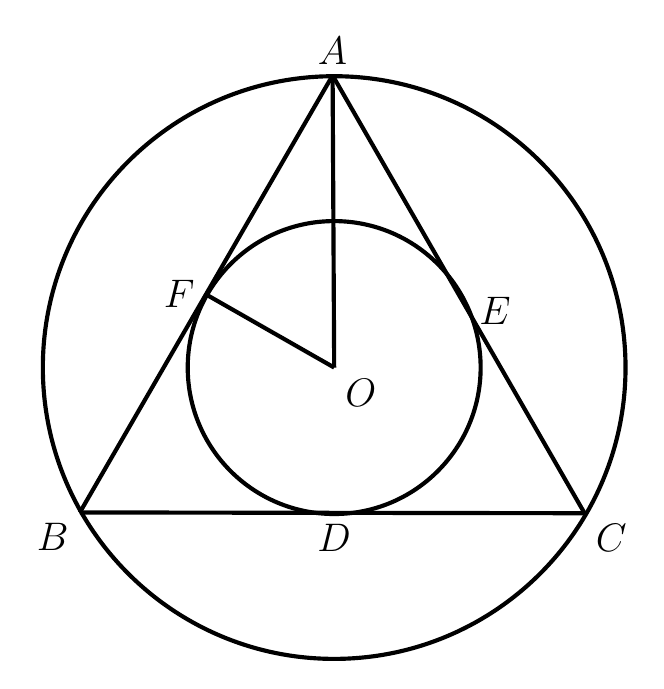
\begin{tikzpicture}[line width=1.5pt, line join=round, font=\fontsize{15.5}{18.6}\selectfont]
  % Named coordinates (converted from pixels)
  \coordinate (A) at (-0.02,3.11);
  \coordinate (B) at (-3.23,-2.44);
  \coordinate (C) at (3.18,-2.45);
  \coordinate (O) at (0,-0.60);
  \coordinate (D) at (0,-2.45);
  \coordinate (E) at (1.70,0.12);
  \coordinate (F) at (-1.63,0.33);

  % Circumcircle and incircle
  \draw (O) circle (3.70);
  \draw (O) circle (1.86);

  % Triangle sides
  \draw (A) -- (B);
  \draw (A) -- (C);
  \draw (B) -- (C);

  % Segment AO and radius OF
  \draw (A) -- (O);
  \draw (O) -- (F);

  % Labels
  \node[above] at (A) {$A$};
  \node[below left] at (B) {$B$};
  \node[below right] at (C) {$C$};
  \node[below] at (D) {$D$};
  \node[right] at (E) {$E$};
  \node[left] at (F) {$F$};
  \node[below right] at (O) {$O$};
\end{tikzpicture}
\end{document}